\documentclass[a4paper,12pt,oneside,bibtotoc,numbers=noenddot]{scrreprt}

%Pakete
\usepackage[latin9]{inputenc}
\usepackage[ngerman]{babel}
\usepackage{listings}
\usepackage{graphicx}
\usepackage{BachelorThesis}

% Allgemeine Informationen
\newcommand\mytitle{Titel der Arbeit}
\newcommand\myauthor{Name des Autors oder der Autoren}
\newcommand\mydepartment{Informatik und Elektrotechnik}
\newcommand\myinstitute{Hochschule Zittau/G\"{o}rlitz}
\newcommand\mytutor{Name und Titel des betreuenden Professors}
\newcommand\mySecondTutor{Name und Titel des betrieblichen Betreuers}

% Abstracts
\newcommand\mysubject{Das deutsche Abstract.}
\newcommand\mysubjectenglish{The english abstract.}

% PDF-Einstellungen
\hypersetup
{
	pdftitle = \mytitle,
	pdfsubject = \mysubject,
	pdfauthor = \myauthor,
	pdfkeywords = {},
	colorlinks = {true},
	pdfborder = 0 0 0
}

\begin{document}
\nocite{*}

%
\pagenumbering{alph}
\begin{titlepage}
\thispagestyle{empty} 
 \begin{center}
 \vspace{2.0cm} 
 {\bfseries \huge Frontend eines Agilent-Parsers erstellen\\}
 \vspace{3.0cm} 
 {\bfseries \huge Belegarbeit\\}
 \vspace{3.0cm}
 {\normalsize eingereicht am Fachbereich\\}
 {\bfseries \Large Informatik\\}
 {\normalsize der Hochschule Zittau/G�rlitz (HAW)\\}
 \vspace{1cm}
 {\normalsize als Pr�fungsleistung im Fach\\}
 {\bfseries \Large Data Mining 2\\}
 \vspace{1cm}
 {\normalsize vorgelegt von:\\}
 {\bfseries \Large Christof Ochmann (35989)\\
 Ingo K�rner (40586)\\}
 \vspace{1cm}
 {\normalsize  G�rlitz, 07. Februar 2013\\}
 \vspace{0.5cm}
 Betreuer:	Prof. ten Hagen\\
 \vfill
\end{center}
\end{titlepage}

%
%% Kurzreferat
\thispagestyle{empty}
\section*{Abstract}\label{Abstract}
In diesem Projekt...

%\mysubject
%\section*{Abstract}
%\mysubjectenglish

\pagenumbering{Roman}
\tableofcontents
\listoffigures
%\lstlistoflistings

\begin{listofacronyms}
\acronym{JVM}{Java Virtual Machine}

\end{listofacronyms}

\begin{flushleft}
\begin{thebibliography}{sotief}
\bibitem{bib1}{Martin, Robert C. (2008): Clean Code: A Handbook of Agile Software Craftsmanship. Prentice Hall International}

\bibitem{bib2}{Freeman, Eric (2007): Entwurfsmuster von Kopf bis Fu�. O'REILLY}

\bibitem{bib3}{\begin{verbatim}http://www.cs.waikato.ac.nz/ml/weka/arff.html (08.06.2012)\end{verbatim}} 



\end{thebibliography}
\end{flushleft}

\newpage
\pagestyle{chapterStyle}
\pagenumbering{arabic}

\chapter{Allgemeines}
\section{Einleitung}\label{Einleitung}
Ziel dieses Projektes ist es, ...
\section{Aufgabenstellung}\label{Aufgabenstellung}
In diesem Projekt sollen gegebene Agilent-Logdateien geparst werden. Aus den geparsten Zeilen soll ein Baum in einem Intermediate-Format erstellt werden. Der erzeugte Baum wird im Hauptspeicher des Rechners gehalten. Die Weiterverarbeitung des Baumes im Intermediate-Format erfolgt in einem anderen Projekt und ist nicht Gegenstand dieser Arbeit. In diesem Projekt muss das Intermediate-Format nicht entworfen werden. Statt dessen wird es von Felix Deutschmann und Daniel Horbach �bernommen. Ein Baum im Intermediate-Format wird immer nur aus einer Agilent-Logdatei erzeugt, d.h. es soll nicht ein Baum aus zwei oder mehreren Agilent-Logdateien erzeugt werden. $Agilent-Logdatei -> Agilent-Parser -> Baum im Intermediate-Format$. 

Das Frontend soll nur Knotennamen ber�cksichtigen, die in den zur Verf�gung stehenden Agilent-Logdateien auch vorkommen. Andere Knotennamen brauchen im Frontend nicht implementiert werden. Treten bei der Verarbeitung einer Agilent-Logdatei einmal unerwartete Knotennamen auf, werden diese in der Datei UnsupportedNodeNames.txt weggeschrieben.

Die Reihenfolge der Kindknoten spielt bei der Erstellung des Baumes keine Rolle.
\section{Relevanz des Forschungsgegenstandes}\label{RelevanzDesForschungsgegenstandes}
Der Forschungsgegenstand dieser Arbeit ist, ein Compiler-Frontend f�r Agilent-Logdateien zu erstellen. Der Forschungsgegenstand ist relevant, da bisher kein Compiler-Frontend f�r das Umwandeln von Agilent-Logdateien in das Intermediate-Format vorliegt. Dar�berhinaus m�ssen f�r das Erstellen des Frontends technische Probleme gel�st werden. Ziel der Forschung ist es, einen Frontend zu entwerfen, dass das Agilent-Logformat in ein Intermediate-Format �berf�hrt.
\section{Der aktuelle Wissensstand}\label{DerAktuelleWissensstand}
Noch nicht vorhandene Kenntnisse �ber das Parsen von Agilent-Logdateien werden aus der Format6.pdf gewonnen. In der Format6.pdf wird das Agilent-Logformat beschrieben.
\chapter{Umsetzung}\label{Umsetzung}
\section{Analyse}\label{Analyse}
In Abbildung \ref{fig:Analyseklassendiagramm} auf Seite \pageref{fig:Analyseklassendiagramm} ist das Analyseklassendiagramm vom Agilent-Parser zu sehen.

\begin{figure}[htp]
\centering
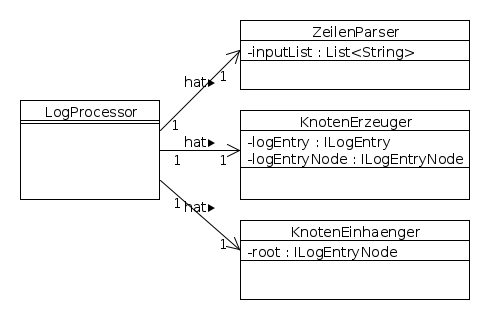
\includegraphics[width=0.6\textwidth]{Ingo/Bilder/Analyseklassendiagramm.png}
\caption{Analyseklassendiagramm Agilent-Parser}
\label{fig:Analyseklassendiagramm}
\end{figure}
\section{Entwurf}\label{Entwurf}
Ziel dieses Projektes ist es, ...

In Abbildung \ref{fig:Entwurfsklassendiagramm} auf Seite \pageref{fig:Entwurfsklassendiagramm} ist das Entwurfsklassendiagramm vom Agilent-Parser zu sehen.

\begin{figure}[htp]
\centering
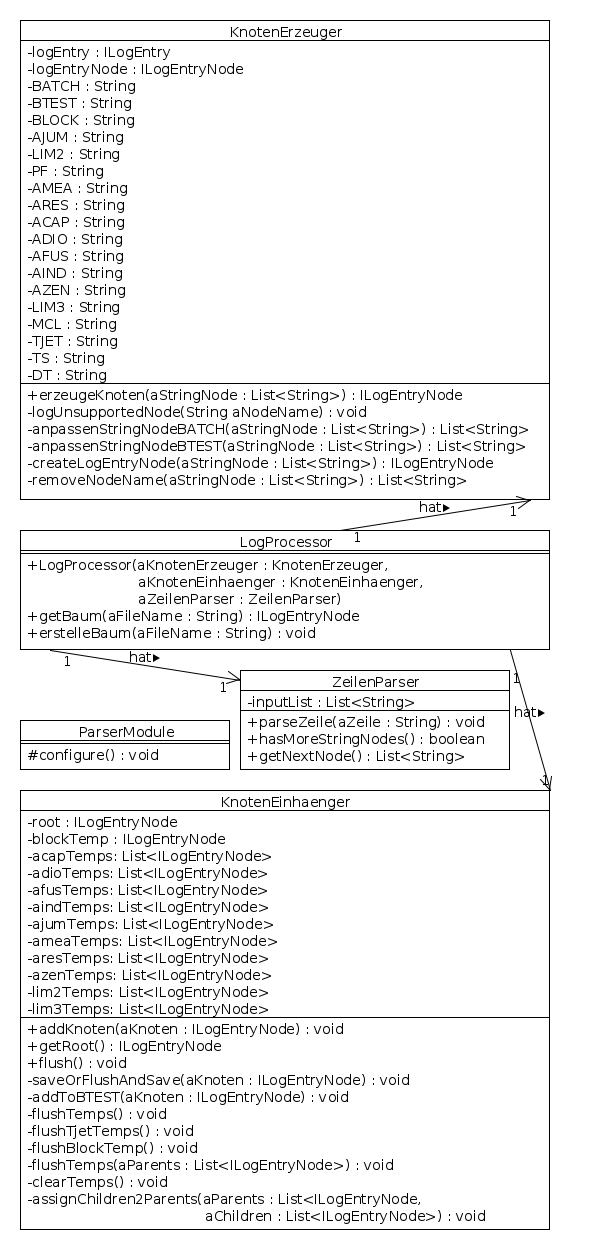
\includegraphics[width=0.6\textwidth]{Ingo/Bilder/Entwurfsklassendiagramm.png}
\caption{Entwurfsklassendiagramm Agilent-Parser}
\label{fig:Entwurfsklassendiagramm}
\end{figure}
\section{Text File Encoding}\label{TextFileEncoding}
Unter Ubuntu 10.04 ist in Eclipse Juno das Text File Encoding standartm��ig auf UTF-8 gesetzt. Die kann beim Kopieren von Stings aus dem Agilent-Logformat zu Fehlern f�hren, da bestimmte UTF-8 Zeichen im Java-Editor unsichtbar sind. Um unsichtbare Zeichen im Java-Editor sichtbar zu machen, sollte unter $Eclipse->Preference->General->Workspace$ das ``Text File Encoding'' von UTF-8 auf ISO-8859-1 umgestellt werden.
\section{Das Agilent-Format}\label{AgilentFormat}
\subsection{Struktur und Syntax}\label{strukturundsyntax}
Testdaten im Agilent-Format  werden in einer Datei als eine Folge von sog. \textit{log-records} gespeichert. Jedes log-record ist durch geschweifte Klammern umschlossen und beginnt mit einen Pr�fix, welches aus einem @-Zeichen besteht, gefolgt von beschreibenden Zeichen, die den Typ des Records eindeutig identifizieren (z.B. @A-JUM). Daraufhin folgt eine bestimmte Anzahl von Datenfeldern, die alphanumerische Messwerte im ASCII-Format enthalten und voneinander durch das \textbar-Zeichen(Pipe) getrennt sind. Sollten einem Datenfeld keine Messwerte zugeordnet worden sein, so wird dies einfach durch zwei nebeneinander stehende Pipes dargestellt(z.B. \textbar \textbar). Falls davon das letzte Datenfeld eines Records betroffen sein sollte, so steht hinter dem letzen Pipe kein weiteres Zeichen(z.B. 501-6338-02\textbar RevA\textbar \textbar \textbar \textbar ) und das Ende des Records wird mit der schlie�enden Klammer ''\}'' markiert oder aber ein neues Subrecord mit der �ffnenden Klammer ''\{'' begonnen.   
Die log-records sind hierarchisch angeordnet in \textit{records} und \textit{subrecords}. Die subrecords dienen dazu  das vorhergehende record genauer zu beschreiben.  Dabei ist jedem subrecord h�chstens ein record unmittelbar �bergeordnet und somit kann man die Log-Datei als einen Baum darstellen um zwischen den einzelnen Knoten zu navigieren und sie auszulesen. \\
Das Wurzelelement jeder der uns zur Verf�gung stehenden Log-Datei ist das \\ @BATCH-Record, welches erst vollst�ndig durch das @BTEST-Record beschrieben wird und dieses als subrecord mit geschweiften Klammern umschlie�t. Jede Log-Datei enth�lt jeweils ein @BATCH-Record und ein @BTEST-Record.  Dies ist die �bliche Struktur  und sie wurde in allen der uns zur Verf�gung stehenden Log-Dateien befolgt. Je nach Testsystem k�nnte es jedoch evtl. zu Abweichungen von dieser Struktur kommen. Es k�nnten beispielsweise mehrere @BATCH-Records in einer Log-Datei gespeichert werden.   
Das @BTEST-Record kann wiederum mehrere subrecords enthalten(siehe FORMAT06.pdf Seite: 6-8), die auch mehrfach in einer Log-Datei vorkommen k�nnen. Ein Beispiel eines h�ufig vorkommenden subrecords von @BTEST w�re @BLOCK.
\subsection{Besonderheiten und Bemerkungen}\label{Besonderheiten}
\begin{itemize}
\item In der Dokumentation des Agilent Data Formats (FORMAT06.pdf) ist @BS-CON als Kind des @BTEST-Records als auch des @BLOCK-Records  aufgef�hrt und taucht in den und zur Verf�gung stehenden Log-Dateien an beiden in Frage kommenden Stellen auf. Um das Problem zu l�sen und @BS-CON einem Knoten eindeutig zuordnen zu k�nnen, m�sste man in jeder Log-Datei herausfinden, ob @BS-CON in der Hierarchie auf derselben H�he steht wie @BLOCK oder ein Kind von @BLOCK ist. 
\item Des Weiteren stimmt die Anzahl der Attribute f�r das @BATCH-Record und f�r das @BTEST-Record in der Dokumentation nicht mit der Legende und auch nicht mit den tats�chlichen Log-Daten �berein.  In der Dokumentation hat @BATCH 13 Attribute, in der Legende und in den Log-Daten jeweils 14 Attribute. Das @BTEST-Record hat 13 Attribute in der Dokumentation und in der Legende, aber in den Log-Daten sind es nur 12.
\item Es existieren mehrere Gruppen von Pr�fixen. Log-records, die beispielsweise mit ''@A'' beginnen, wurden mit analogen Test-statements, und die, die mit ''@D'' beginnen, wurden mit digitalen Test-statements erzeugt. 
\item Jedes @BTEST sowie jedes @BLOCK-Record und alle Records, die auf der selben Hierarchiestufe angesiedelt sind beginnen in einer neuen Zeile der Log-Datei.
\item Die Datenfelder zwischen den Pipes k�nnen von folgenden Typ sein: 
\begin{itemize}
\item Boolean (1 oder 0)
\item Flie�kommazahl(z.B. 1.0253+E01)
\item Integer(z.B. -125)
\item String(z.B. Node14, +5Volts o.�.) 
\item Null-Zeichen (Ein leeres Datenfeld enth�lt kein einziges Zeichen zwischen zwei Pipes. Dabei ist zu beachten, dass hinten dem letzten Pipe sich immer noch ein Datenfeld befindet, das keine Werte enth�lt.) 
\end{itemize}
\end{itemize}



\section{Unstimmigkeiten im Agilent-Format}\label{UnstimmigkeitenImAgilentFormat}
In der Format06.pdf auf Seite 35 stimmt bei BATCH die Anzahl der Attribute nicht mit der Legende �berein. Auch in den tats�chlichen Agilent-Logdateien stimmt die Anzahl der Attribute nicht immer mit der Anzahl der Attribute �berein, wie sie in der Format06.pdf beschrieben werden.

In der Format06.pdf auf Seite 40 stimmt bei BTEST die Anzahl der Attribute nicht immer mit der tats�chlich vorkommenden Anzahl in der Agilent-Logdatei �berein.
\section{Unit Tests}\label{UnitTests}
\subsection{ZeilenParserTest}
Im ZeilenparserTest werden die Methode \textit{parseZeile()}, \textit{hasMoreStringNodes()} sowie \textit{getNextNode()} getestet. Zuerst wird der Methode parseZeile() eine Zeile der Log-Datei als String �bergeben z.B.:
\begin{verbatim}
{@BATCH|501-6338-02|50|12|1||btest|040107103921||solmb3t1|||||
\end{verbatim}
Daraufhin werden alle geschweiften Klammern aufgel�st und die einzelnen Parameter in einer List$<$String$>$ gespeichert. Die Methode hasMoreStringNodes() liefert true, falls ein Listenelement den Anfang eines Records darstellt und mit @-Zeichen beginnt. Wenn eine Zeile mehrere Records enth�lt, wird mit getNextNode() immer das komplette n�chste Record als Liste zur�ckgegeben. Diese Funktionalit�t wird beispielsweise in folgendem Test gepr�ft:
\begin{verbatim}
@Test
	public void testGetNextSecond() {
		String inpu = "{@A-JUM|0|+7.630803E+06{@LIM2|+9.999999E+99|+1.000000E+04}}";
		zeilenParser.parseZeile(inpu);
		zeilenParser.getNextNode();
		ArrayList<String> stringNode = new ArrayList<String>();
		stringNode.add("@LIM2");
		stringNode.add("+9.999999E+99");
		stringNode.add("+1.000000E+04");
		assertTrue(zeilenParser.getNextNode().equals(stringNode));
	} 
\end{verbatim}
\subsection{KnotenErzeugerTest}
Im KnotenErzeugerTest wird die Methode \textit{erzeugeKnoten()} getestet. Ihr wird eine Liste mit den Attributen eines Records �bergeben, die mit Hilfe der \textit{NodeCreatorUtil}-Klasse erzeugt wurde. Daraufhin pr�ft die Methode anhand des ersten Listenelements um welches Record es sich handelt und erzeugt eine Instanz der entsprechenden Record-Klasse, die eine Implementierung der \textit{ILogEntry}-Schnittstelle ist. Jede Record-Instanz enth�lt die beiden Listen \textbf{headings} und \textbf{values}. Headings sind die Namen der Record-Attribute und werden im Konstruktor gesetzt. Anschlie�end ruft die \textit{erzeugeKnoten()}-Methode createLogEntryNode() auf, in der die values gesetzt werden und eine Instanz der \textit{LogEntryNode-Klasse} erzeugt wird. Im Unit-Test wird gepr�ft, ob der richtige Knoten erfolgreich erzeugt wurde:
\begin{verbatim}
@Test
	public void testErzeugeKnotenBATCH() {
		ILogEntryNode logEntryNode = testNodeCreator.createNodeBATCH();
		assertEquals(BATCH.class, logEntryNode.getLogEntry().getClass());
	}
\end{verbatim}

\subsection{KnotenEinhaengenTest}
Hierbei wird die Methode \textit{addKnoten()} getestet. Nachdem ein Knoten erzeugt wurde, wird er ihr als Parameter �bergeben. Diese pr�ft zuerst um welchen Knoten-Typ es sich handelt. Wenn es ein BATCH-Knoten ist, wird er zum Wurzelknoten(root) des Baumes. Der BTEST-Knoten wird mit \textit{root.getSubNodes().add(knoten)} an den Wurzelknoten eingeh�ngt. Folgt anschlie�end ein BLOCK-Knoten, werden zuerst an alle seine Unterknoten deren Kinder eingeh�ngt und zum Schluss wird der BLOCK-Knoten in \textit{flushBlockTemp()} an den BTEST-Knoten angef�gt. 
Im KnotenEinhaengenTest werden zuerst der Reihe nach die gew�hlten Knoten an das Wurzelelement mit addKnoten() eingeh�ngt um anschlie�end ein bestimmtes Element herauszulesen:
\begin{verbatim}
@Test
	public void testAddKnotenBATCH_BTEST_BLOCK_AJUM() {
		knotenEinhaenger.addKnoten(testNodeCreator.createNodeBATCH());
		knotenEinhaenger.addKnoten(testNodeCreator.createNodeBTEST());
		knotenEinhaenger.addKnoten(testNodeCreator.createNodeBLOCK());
		knotenEinhaenger.addKnoten(testNodeCreator.createNodeAJUM());
		knotenEinhaenger.flush();
		ILogEntryNode node = knotenEinhaenger.getRoot();
		ILogEntryNode batch = node;
		ILogEntryNode btest = batch.getSubNodes().get(0);
		ILogEntryNode block0 = btest.getSubNodes().get(0);
		ILogEntryNode block0_ajum = block0.getSubNodes().get(0);
		assertEquals(AJUM.class, block0_ajum.getLogEntry().getClass());
	}
\end{verbatim}

%\chapter{Theoretische Grundlagen}
%Die f\"{u}r den Untersuchungsgegenstand relevanten Themen, die \"{u}ber die
%grundlegenden Studieninhalte hinausgehen; oft auch anwendungsspezifische Aspekte - %ca. 6 Seiten

%\chapter{Ist-Analyse}
%Welche Defizite sollen mit der Arbeit behoben werden, welche nicht? %Pr\"{a}zisierung
%der Zielstellung - ca. 6 Seiten

%\chapter{L\"{o}sungskonzept}
%Wie sollen die Defizite behoben werden? Methoden, fachliche Auseinandersetzung
%mit alternativen Ans\"{a}tzen und Auffassungen, Systembeschreibung (Architektur,
%Vorgehensmodell, \ldots) - ca. 12 Seiten

%\chapter{Implementierung}
%Umsetzung des L\"{o}sungskonzepts, Begr\"{u}ndung der verwendeten Technologien - %ca. 8
%Seiten

%\chapter{Ergebnisse}
%Objektive Bewertung der vorliegenden L\"{o}sung, diverse Testverfahren,
%Nutzerbefragungen - ca. 4 Seiten

%\chapter{Fazit und Ausblick}
%Zusammenfassung s\"{a}mtlicher Ergebnisse in Bezug auf die Zielerf\"{u}llung und
%Vorschl\"{a}ge f\"{u}r weiterf\"{u}hrende Arbeiten - ca. 2 Seiten

\bibliographystyle{alphadin}
\begin{appendix}
\newpage
\pagestyle{appendixAStyle}
%\chapter{Codebeispiele}
%\input{listings}
\end{appendix}

\newpage
\chapter{Arbeitsaufteilung}


\begin{table}[h] \begin{flushleft}  \begin{tabular}{|l||c|c|c|c|c|c|}
\hline
\textbf{Arbeit}		&	\textbf{C. Ochmann}	& \textbf{I. K�rner}  \\ \hline \hline
Abstract   	      &                     & 0       \\
Einleitung  &                             		      & ~\ref{Einleitung} \\
Aufgabenstellung&                                  & ~\ref{Aufgabenstellung}  \\
Forschungsgegenstand&                              & ~\ref{RelevanzDesForschungsgegenstandes} \\ 
akt. Wissensstand&                                      & ~\ref{DerAktuelleWissensstand}  \\ 
Hintergrund&                                      & ~\ref{Hintergrund}  \\ 
Analyse&                                      & ~\ref{Analyse}  \\ 
Funktionale Anforderungen&                                      & ~\ref{FunktionaleAnforderungen}  \\ 
Nichtfunktionale Anforderungen&                                      & ~\ref{NichtfunktionaleAnforderungen}  \\ 
Entwurf&                                      & ~\ref{Entwurf}  \\ 
Struktur und Syntax& ~\ref{strukturundsyntax} &										\\
Besonderheiten und Bemerkungen&  ~\ref{Besonderheiten}    &     \\
Entwicklungsumgebung&                                      & ~\ref{Entwicklungsumgebung}  \\ 
Dependency Injection mit Goolge Guice&                                      & ~\ref{DependencyInjectionMitGoogleGuice}  \\ 
Projekt importieren&                                      & ~\ref{ProjektImportieren}  \\ 
Projekt ausf�hren&                                      & ~\ref{ProjektAusfuehren}  \\ 
ZeilenParserTest&   ~\ref{zeilenparsertest}          &  \\
KnotenErzeugerTest&   ~\ref{knotenerzeugertest}          &  \\
KnotenEinhaengenTest&   ~\ref{knoteneinhaengentest}          &  \\
Funktionale Tests&                                      & ~\ref{FunktionaleTests}  \\ 
Zusammenfassung&                                      & ~\ref{Zusammenfassung}  \\ 
\hline \hline
\end{tabular} \end{flushleft} \caption{Aufteilung} \end{table}



\newpage
\chapter{Eigenst�ndigkeitserkl�rung}
Hiermit erkl�re ich, dass ich diese Arbeit selbst�ndig verfasst habe. Mir ist bekannt, dass jede Form des Plagiats mit der Note 5 (Betrugsversuch) bewertet wird.

\begin{tabular}{@{}p{6.0cm}p{6.0cm}}	  		  		 	
	  		 & \\
	  		 & \\
				  			\textbf{Ochmann, Christof} &               Unterschrift:\\				 
				 &\\
				 & \\
				  			\textbf{K�rner, Ingo}   	&                     Unterschrift:\\			
\end{tabular}
\end{document}
